\section{Key insights and ideas}

As stated in previous section, the biggest challenge of optimizing user-perceived quality is that perceived quality is related to both video content and user behavior. To solve the challenge, we show that perceived quality optimization can be decoupled: we can optimize video-content-related factors on server-side and optimize user-behavior-related factors on client-side.

\subsection{Insights}
In this section, we show that in VR streaming, each visual factor influences user-perceived quality independently. So we can decouple them into several single factors to measure perceived quality respectively, then we design an server-side offline tiling scheme only with consideration of video content, and design a client-side bitrate allocation method only with consideration of user behavior.

\textbf{Insight 1: Perceived quality model in VR display can be built by simply adding several new factors on traditional perceived quality model.}

In traditional video display, there are many factors which influence user-perceived quality. Prior works have studied how single factors influence user-perceived quality. Moreover, \cite{distance} proves that, in perceived quality computation, several factors (luminance, texture complexity, etc.) can be considered independently. As a result, we can independently measure the influence of each factor as a coefficient, and multiply them together to obtain the final user-perceived quality.

However, in VR display, there are some new factors which are never considered in traditional video display. So how these new factors, together with factors in traditional video display, influence the perceived quality in VR streaming, is an unknown problem. We intend to assume that they can also be computed independently, and then multiplied as coefficients together with traditional factors to obtain final user-perceived quality.

To prove our guess, we set up a user study to evaluate how perceived quality is influenced by multiple factors. (Sec. 4) Our result shows that perceived quality model in VR display can be decoupled. We only need to simply add new factors to traditional perceived quality model.

\textbf{Insight 2: Video tiling strategy can be optimized on server side.}

In traditional grid-like video tiling scheme, video is cut into m*n rectangular tiles with equal size. 

This tiling strategy has an obvious drawback: at most times the boundary between objects are not exactly on the boundary between two adjacent tiles. Fig. \ref{fig_insight_tiling} shows an example. In the video frame, there are two objects (Object A, Object B) and a background. In coarse-grained tiling (Fig. \ref{fig_insight_tiling}(b)), the object can not be exactly caught by one or several tiles. It leads to bitrate allocation of low performance. In fine-grained tiling (Fig. \ref{fig_insight_tiling}(c)), although the object can be caught by several tiles, it cut the video into too many tiles and many cutting lines are unnecessary. It leads to serious bandwidth efficiency problem as described in Sec. 2.3.

\begin{figure*}[!t]  
\begin{tabular}{cccc}  
\begin{minipage}[t]{0.24\linewidth}  
 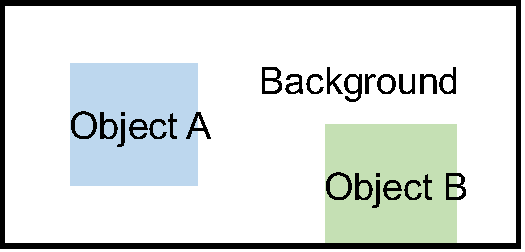
\includegraphics[width = 1\linewidth]{images/insight_tiling1.pdf}  
     \center{(a) A video frame.}
     \label{fig_insight_tilinga}
\end{minipage}  
\begin{minipage}[t]{0.24\linewidth}  
    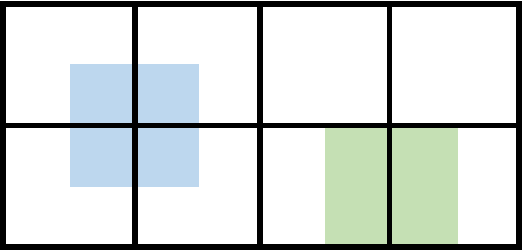
\includegraphics[width = 1\linewidth]{images/insight_tiling2.pdf}  
     \center{(b) Grid-like tiling in coarse granularity.}
     \label{fig_insight_tilingb}
\end{minipage}  
\begin{minipage}[t]{0.24\linewidth}  
 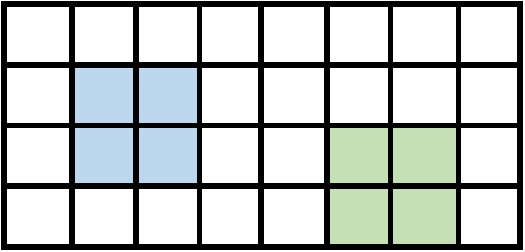
\includegraphics[width = 1\linewidth]{images/insight_tiling3.pdf}  
     \center{(c) Grid-like tiling in fine granularity.}
     \label{fig_insight_tilingc}
\end{minipage}  
\begin{minipage}[t]{0.24\linewidth}  
 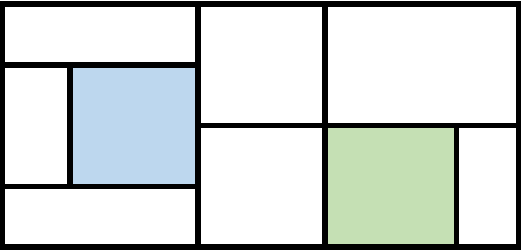
\includegraphics[width = 1\linewidth]{images/insight_tiling4.pdf}  
     \center{(d) Object-based tiling.}
     \label{fig_insight_tilingd}
\end{minipage}  
\end{tabular}  
  \caption{An example of traditional grid-like tiling and object-based tiling.}  
\label{fig_insight_tiling}
\end{figure*}  

Suppose we can know information about video content, we can cut the video based on objects like Fig. \ref{fig_insight_tiling}(d). In this method, we can obtain similar tiling granularity as Fig. \ref{fig_insight_tiling}(c) but remain similar tile numbers as Fig. \ref{fig_insight_tiling}(b). We think tiling scheme like Fig. \ref{fig_insight_tiling}(d) can outperform traditional grid-like tiling scheme. Moreover, since information of objects is only related to video content, it is totally independent from user. So object-based tiling can be completed offline on server-side.

\textbf{Insight 3: Perceived quality computation can be decoupled.}

Although accurately computing perceived quality needs the information of both video content and actual user behavior, we can precompute perceived quality of given video content with each possible user behavior situations on server-side, without any information of actual user behavior, and transform the computation result to client. Client only needs to choose the situation which match actual user behavior most, then uses given perceived quality value to approximate the actual perceived quality. Experimental results prove that we can obtain very good approximation accuracy with very little end-to-end exchanging overhead of computation result transforming. 

\subsection{Key ideas to solve the challenges}

Based on above insights, we decouple the visual characteristics due to video content and user viewpoint, and design a perceived quality driven VR streaming system which consider visual characteristics of video objects completely on server-side, and considers visual characteristics of user behavior completely on client-side. Specifically, we build our system based on following ideas:

\begin{itemize}

\item \emph{Measuring perceived quality in VR streaming by incrementally adding some new coefficients into traditional non-VR perceived quality model.} (\S 4)

\item \emph{Server-side offline video tiling only based on of video content.} (\S 5)

\item \emph{Server-side perceived quality precomputation and client-side approximation \& optimization.} (\S 6)

\end{itemize}
